\section{Intelligence Artificielle}

\subsection{CNN Multi-labels}

Pour déterminer les emplacements réels des dégradations sur la route, nous avons utilisé une méthode de fenêtre glissante sur les séquences accélérométriques \cite{fenetre_glissante}

\subsection {Localisation GPS des détériorations}

\subsubsection{Liaison entre les Dégradations Détectées et les Données GPS}

Cette approche de fenêtre glissante nous permet de localiser précisément les instants dans lesquels des dégradations ont été détectées. Les indices de ces détections sont stockés dans la liste \texttt{all\_predicted\_indices}.\\

Par la suite, nous avons associé ces indices aux données GPS recueillies simultanément avec les données accélérométriques. Chaque indice correspond à un enregistrement au même moment, reliant ainsi les détections de dégradations aux coordonnées géographiques respectives.\\

Pour visualiser ces emplacements sur une carte, nous avons utilisé la bibliothèque Folium \cite{folium}. Les coordonnées GPS associées aux indices détectés ont été enregistrées dans un fichier CSV (\texttt{detected\_gps\_data.csv}). Les premières entrées de ce fichier ont été modifiées à des fins de test, en utilisant les coordonnées de la ville d'Illkirch \cite{gps_site}:\\

\begin{figure}[H]
    \centering
    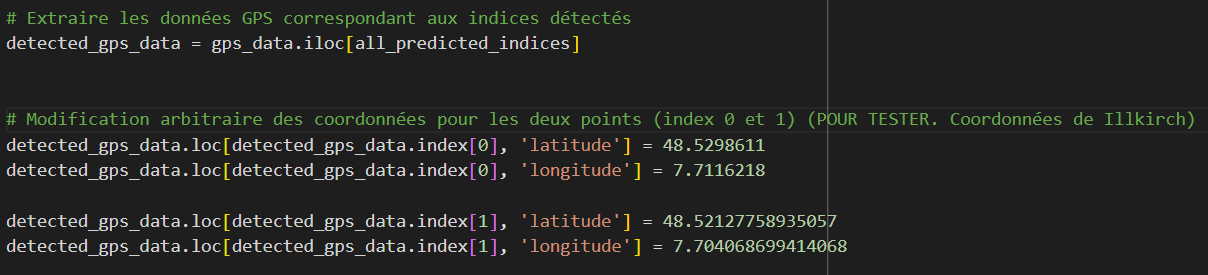
\includegraphics[width=0.9\linewidth]{img/gps_a_la_main.png}
    \caption{Modification arbitraire des données GPS (test)}
\end{figure}

Enfin, une carte interactive a été générée, centrée sur le premier point GPS associé à une détection. Des marqueurs ont été ajoutés à chaque position GPS détectée, offrant ainsi une représentation visuelle des endroits où les dégradations ont été identifiées.\\

\begin{figure}[H]
    \centering
    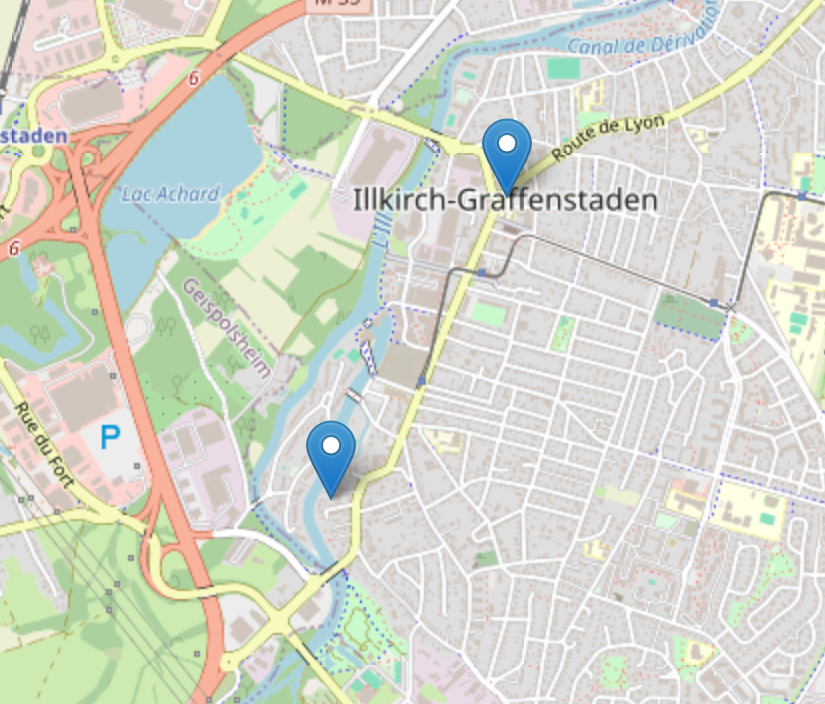
\includegraphics[width=0.5\linewidth]{img/gps_test_illkirch.png}
    \caption{Visualisation des données GPS arbitraires sur la carte}
\end{figure}

L'objectif prochain est d'établir un moyen interactif de visualisation de cette carte.